\chapter{System Implementation}
\label{ch:system-implementation}

This chapter describes how the design developed in Chapter~3 is realised in
the prototype. The discussion begins with the build artefacts and then follows
the mechanisms that construct, load, transport, decode, select and interpret
runtime observations. Each mechanism is described in its primary location;
later sections refer to that implementation rather than restating the complete
event lifecycle. Experimental behaviour and performance measurements are
reserved for Chapter~5.

\section{Build Toolchain and Project Organisation}
\label{sec:implementation-build-organisation}

The build process consists of three ordered stages. First, the libbpf source in
\path{3rdparty/libbpfgo/libbpf/src} is compiled locally into the static library
\path{dist/libbpf/obj/libbpf.a}, together with the required headers and package
metadata. Second, Clang compiles the eBPF source into
\path{dist/project.bpf.o} for the x86-64 target. Finally, the Go application is
built through CGO using the local libbpf library and libbpfgo bindings, producing
the executable \path{dist/project}. The Makefile preserves this order and
ensures that all stages use the dependencies included in the repository rather
than system-installed versions.

The eBPF object is also embedded in the Go executable. For this reason,
\path{dist/project.bpf.o} must be generated before the Go build starts. At
runtime, the application can load the embedded object without requiring a
separate copy beside the executable. Developers may still provide an external
object through the command-line configuration for testing or compatibility
analysis. The executable nevertheless remains dependent on the host kernel,
its BTF data, the required privileges and the system libraries used by CGO.

\section{eBPF Program Implementation}
\label{sec:implementation-ebpf-programs}

The eBPF object contains programs attached to different kernel hook types. Most
of these programs produce records in one of two ways. A direct producer creates
and submits an event during a single hook invocation. A paired producer saves
the request arguments when an operation begins and completes the event when a
return hook provides its result.

Physical hooks and public events do not have a one-to-one relationship. Several
eBPF programs may contribute to the same logical event and use the same event
schema. Conversely, some attached programs only provide internal support and
do not generate a public event. Section~\ref{sec:implementation-loader-registry}
explains how the loader translates these relationships into an attachment plan.


\subsection{Shared Event-Construction Framework}
\label{subsec:implementation-shared-event-construction}

Both construction forms use a per-CPU workspace to build events. Each CPU has
its own reusable record, avoiding the need to place the complete event structure
on the limited eBPF stack. Additional per-CPU maps provide temporary storage
for path reconstruction and intermediate kernel objects, while task and process
maps retain context that can be reused across hook invocations.

The common initialisation helper clears the argument buffer and records the
basic identity and timing information. Each hook then appends its
event-specific fields. Immediately before submission, the common submission
helper updates the complete task context and sends the record through the
kernel-to-user-space interface described in
Section~\ref{sec:implementation-binary-contract}.

Listing~\ref{lst:ebpf-shared-construction} shows the main stages shared by these
helpers. Details related to process-map initialisation and optional stack
capture are omitted because they do not change the event-construction process.

\newpage

\begin{lstlisting}[
      language=C,
      basicstyle=\ttfamily\footnotesize,
      caption={Shared event construction and submission path.},
      label={lst:ebpf-shared-construction}
  ]
  if (!p->event)
      p->event = bpf_map_lookup_elem(&event_data_map, &zero);
  if (!p->event)
      return 0;

  p->config = bpf_map_lookup_elem(&config_map, &zero);
  if (!p->config)
      return 0;

  reset_event_args_buf(p->event);
  p->event->task = (struct task_struct *) bpf_get_current_task();

  u64 id = bpf_get_current_pid_tgid();
  p->event->context.task.host_tid = id;
  p->event->context.task.host_pid = id >> 32;
  p->event->context.eventid = event_id;

  init_task_context(&p->event->context.task,
                    p->event->task, p->config->options);

  u32 size = sizeof(event_context_t) + sizeof(u8) +
             p->event->args_buf.offset;
  long ret = bpf_perf_event_output(
      p->ctx, &events, BPF_F_CURRENT_CPU, p->event, size);

  update_event_stats(p->event->context.eventid, ret);
  return ret;
  \end{lstlisting}

The per-CPU workspace is reused after each event submission. When the
submission helper is called, the completed portion of the record is copied to
the perf-event channel, so later modifications to the workspace do not affect
the submitted event. If the program cannot obtain the required workspace,
configuration or task context, it stops processing that invocation without
producing a record.

The complete implementation also verifies the record size before submission
and optionally updates delivery statistics. The listing therefore focuses on
the point at which the event leaves kernel space. The precise size checks and
error-handling rules are described in
  Section~\ref{sec:implementation-binary-contract}.

Paired producers build one event across two hook invocations. The entry program
stores the request arguments in a shared map, while the return program retrieves
them and adds the operation result. Each map entry is identified by the logical
event and the host thread that issued the request. This allows the return hook
to recover the correct arguments without mixing different operations performed
by the same thread.

\begin{lstlisting}[
      language=C,
      basicstyle=\ttfamily\footnotesize,
      caption={Saving and recovering arguments for paired producers.},
      label={lst:ebpf-entry-state}
  ]
  statfunc u64 get_args_id(u32 event_id)
  {
      return ((u64) event_id << 32) |
             (u32) bpf_get_current_pid_tgid();
  }

  statfunc int save_args(args_t *args, u32 event_id)
  {
      u64 key = get_args_id(event_id);
      bpf_map_update_elem(&args_map, &key, args, BPF_ANY);
      return 0;
  }

  statfunc int load_args(args_t *args, u32 event_id)
  {
      u64 key = get_args_id(event_id);
      args_t *saved = bpf_map_lookup_elem(&args_map, &key);
      if (!saved)
          return -1;

      /* Fixed argument-slot copies are omitted. */
      return 0;
  }
\end{lstlisting}

Including the event identifier in the key prevents different paired operations
from using the same map entry. The implementation copies the seven argument
slots explicitly, keeping every memory access statically bounded for the eBPF
verifier. If no entry is found, the return program cannot reconstruct the
event and therefore produces no record.

After the saved arguments have been copied, the return program removes the map
entry and appends the operation result. New entry data is stored with
\texttt{BPF\_ANY}, allowing it to replace stale state left by a missing return
hook. The map is therefore temporary correlation storage, not a history of
process activity.

The following subsections apply these two construction patterns to different
hook families. The interpretation of each event depends on where the hook is
placed within the kernel operation. A syscall-entry hook records the operation
requested by a process, but not its outcome. A security hook observes the
operation while it is being checked by the kernel, without necessarily
revealing the final decision. A committed-state hook runs after a new state has
been installed, while a lifecycle tracepoint reports that a process transition
has occurred. An exit or return hook completes the observation by recording the
result available at that boundary, such as a returned value or error code.

\subsection{Process Lifecycle and Executable Transitions}
\label{subsec:implementation-process-execution-hooks}

Process monitoring must distinguish between a creation request and the
lifecycle transition produced by the kernel. Syscall events expose the
operation selected by the process and the result returned at the syscall
boundary. Scheduler tracepoints instead observe tasks that have already been
created, renamed or terminated. The implementation combines these sources
because neither view is sufficient on its own.

\subsubsection{Process Creation and Lifecycle}

The \texttt{fork} and \texttt{vfork} events provide the simplest syscall-level
view of process creation. Their schemas contain only the return value, so their
entry probes do not retain any arguments. A positive result identifies the
child returned to the caller, while a negative result records the reported
error.

The \texttt{clone} event captures a more configurable creation request. Its
entry probe retains the clone flags, stack address, parent and child thread-ID
pointers, and thread-local-storage value. These fields describe which resources
the new task should share with its parent and where its execution context
should be initialised. The exit probe combines them with the returned child
identifier or error. The resulting event therefore preserves both the requested
creation model and the syscall outcome.

Syscall results alone do not provide the complete parent-child state observed
by the scheduler. The \texttt{sched\_process\_fork} tracepoint runs after the
child task has been created and receives both task structures. It records the
host PID and TID of the parent and child, together with the child's start time.
Listing~\ref{lst:sched-process-fork-evidence} shows the extraction of this
effect-level evidence.

\begin{lstlisting}[
    language=C,
    basicstyle=\ttfamily\footnotesize,
    caption={Parent-child evidence collected by
    \texttt{sched\_process\_fork} (abridged).},
    label={lst:sched-process-fork-evidence}
]
struct task_struct *parent =
    (struct task_struct *) ctx->args[0];
struct task_struct *child =
    (struct task_struct *) ctx->args[1];

u32 parent_pid = get_task_host_tgid(parent);
u32 parent_tid = get_task_host_pid(parent);
u32 child_pid = get_task_host_tgid(child);
u32 child_tid = get_task_host_pid(child);
u64 child_start = get_task_start_time(child);

save_to_submit_buf(&p.event->args_buf,
                 &parent_pid, sizeof(u32), 0);
save_to_submit_buf(&p.event->args_buf,
                 &parent_tid, sizeof(u32), 1);
save_to_submit_buf(&p.event->args_buf,
                 &child_pid, sizeof(u32), 2);
save_to_submit_buf(&p.event->args_buf,
                   &child_tid, sizeof(u32), 3);
save_to_submit_buf(&p.event->args_buf,
                   &child_start, sizeof(u64), 4);
\end{lstlisting}

The start time complements the numeric child identifiers. PIDs and TIDs may be
reused after a task terminates, while the start time allows user space to
distinguish separate task lifetimes associated with the same identifier. This
combination also provides a stronger process identity for local detector
correlation.

Two direct tracepoints cover later lifecycle changes.
\texttt{task\_rename} records the previous and new command names when the task
name changes. This operation is kept separate from executable replacement
because a command-name change does not imply that a new program image was
installed. The \texttt{sched\_process\_exit} event records the task's exit code
and whether the complete thread group is terminating, distinguishing a single
thread exit from the end of the process.

The implementation emits these lifecycle relations as bounded events rather
than maintaining a persistent process graph in kernel space. Syscall events
describe requests and returned outcomes, whereas scheduler tracepoints provide
evidence of task states visible after the corresponding kernel transition.
Longer-lived reconstruction remains a user-space responsibility.

\subsubsection{Executable Transitions}

Executable-transition monitoring must preserve both the program requested by a
process and the outcome of the replacement operation. The pathname and
arguments available at syscall entry describe the process's intention, but they
cannot establish whether the kernel accepted the executable or installed the
new image. The implementation therefore observes the request, binary security
processing and final outcome at separate kernel boundaries.

\begin{figure}[H]
    \centering
    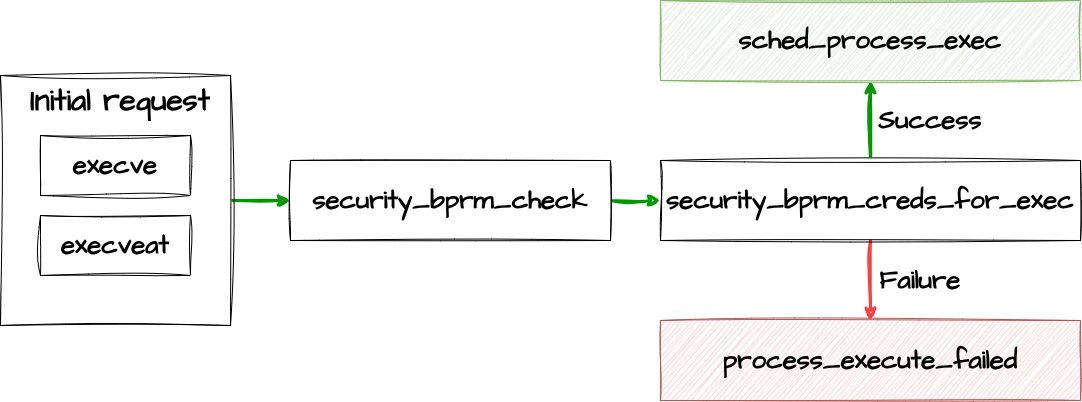
\includegraphics[
        width=0.85\textwidth,
        keepaspectratio
    ]{figures/chapter4/execution_monitoring.drawio.png}
    \caption[Execution monitoring: attempts and outcomes]
    {Events used to observe execution requests, kernel security processing
    and executable-transition outcomes.}
    \label{fig:execution-monitoring}
\end{figure}

Figure~\ref{fig:execution-monitoring} represents monitoring coverage rather
than a guaranteed one-to-one event sequence. Binary-handler and interpreter
processing may cause security-stage observations to occur more than once.
Furthermore, the security hooks identify intermediate kernel processing but do
not expose the final security decision.

The initial request is captured through \texttt{execve} and
\texttt{execveat}. Both events preserve the requested pathname and up to 38
argument strings while the original user-space memory is still available.
The \texttt{execveat} event additionally records the directory file descriptor
and execution flags, which are required to interpret relative paths and
descriptor-based execution. These events are emitted at syscall entry and
therefore do not contain an execution result.

The \texttt{security\_bprm\_check} hook observes the executable after the
kernel has constructed its \texttt{linux\_binprm} representation. At this
stage, the implementation can record the resolved pathname, device and inode,
original filename, argument count and environment count. These fields associate
the request with a resolved kernel object rather than relying only on the
caller-supplied path.

The \texttt{security\_bprm\_creds\_for\_exec} hook provides a related view of
credential preparation. It captures the same binary identity fields and adds
the file change time. This observation does not prove that the prepared
credentials became active; committed credential transitions are monitored
separately by the mechanism described in
Section~\ref{subsubsec:implementation-identity-credentials}.

The final outcome is represented by two mutually exclusive logical events.
A \texttt{sched\_process\_exec} event confirms that the process installed a new
executable image and records its resolved filename. An unsuccessful
\texttt{execve} or \texttt{execveat} instead produces
\texttt{process\_execute\_failed}, which retains the operation variant,
directory file descriptor, requested pathname, flags and negative return value.

The failure event uses paired entry and exit programs because the pathname and
execution options are available before the syscall runs, while the error is
available only when it returns. Listing~\ref{lst:process-execute-failed}
shows the return-side selection that suppresses successful executions.

\begin{lstlisting}[
    language=C,
    basicstyle=\ttfamily\footnotesize,
    caption={Return-side emission of failed executable transitions
    (abridged).},
    label={lst:process-execute-failed}
]
args_t args = {};
if (load_args(&args, PROCESS_EXECUTE_FAILED) != 0)
    return 0;

del_args(PROCESS_EXECUTE_FAILED);

if (ret >= 0)
    return 0;

program_data_t p = {};
if (!init_program_data(&p, ctx, PROCESS_EXECUTE_FAILED))
    return 0;

int operation = (int) args.args[0];
int dirfd = (int) args.args[1];
const char *pathname = (const char *) args.args[2];
int flags = (int) args.args[3];

save_to_submit_buf(&p.event->args_buf,
                   &operation, sizeof(operation), 0);
save_to_submit_buf(&p.event->args_buf,
                   &dirfd, sizeof(dirfd), 1);
if (pathname)
    save_str_to_buf(&p.event->args_buf, pathname, 2);
save_to_submit_buf(&p.event->args_buf,
                   &flags, sizeof(flags), 3);
save_to_submit_buf(&p.event->args_buf,
                   &ret, sizeof(ret), 4);

return events_perf_submit(&p);
\end{lstlisting}

The saved entry state is removed before the return value is evaluated. A
successful result therefore clears the temporary map entry without generating
a failure record, while a negative result is serialised with the original
request. Separate entry and exit programs handle \texttt{execve} and
\texttt{execveat}, but all four physical programs converge on the same public
event schema.

This design keeps caller intent, resolved binary identity and observed outcome
as distinct forms of evidence. It avoids interpreting an execution attempt as
a successful transition and allows user space to present negative return values
as readable execution errors.

\subsection{Identity, Credentials, Process Control and Limits}
\label{subsec:implementation-identity-control-hooks}

\subsubsection{Identity and Credentials}
\label{subsubsec:implementation-identity-credentials}

A privilege transition cannot be reconstructed reliably from a set-ID syscall
alone. The syscall identifies the change requested by the process and reports
its result, but credentials may also change during executable loading or
through internal kernel paths. Conversely, a security hook exposes a proposed
transition without proving that the new state became active. The implementation
therefore separates requested identity changes, security mediation, committed
credentials and subsequent capability checks.

Linux associates each process with several user and group identifiers. The
real ID represents the identity under which the process was started, while the
effective ID is used for most access-control decisions. The saved ID allows a
process to retain an effective identity that may later be restored, supporting
temporary privilege reduction and recovery. Linux also maintains filesystem
IDs, which are used specifically during filesystem permission checks. The same
distinction applies to user and group credentials \cite{gazestani2025linuxuids}.

\begin{figure}[H]
    \centering
    \makebox[\textwidth][c]{%
        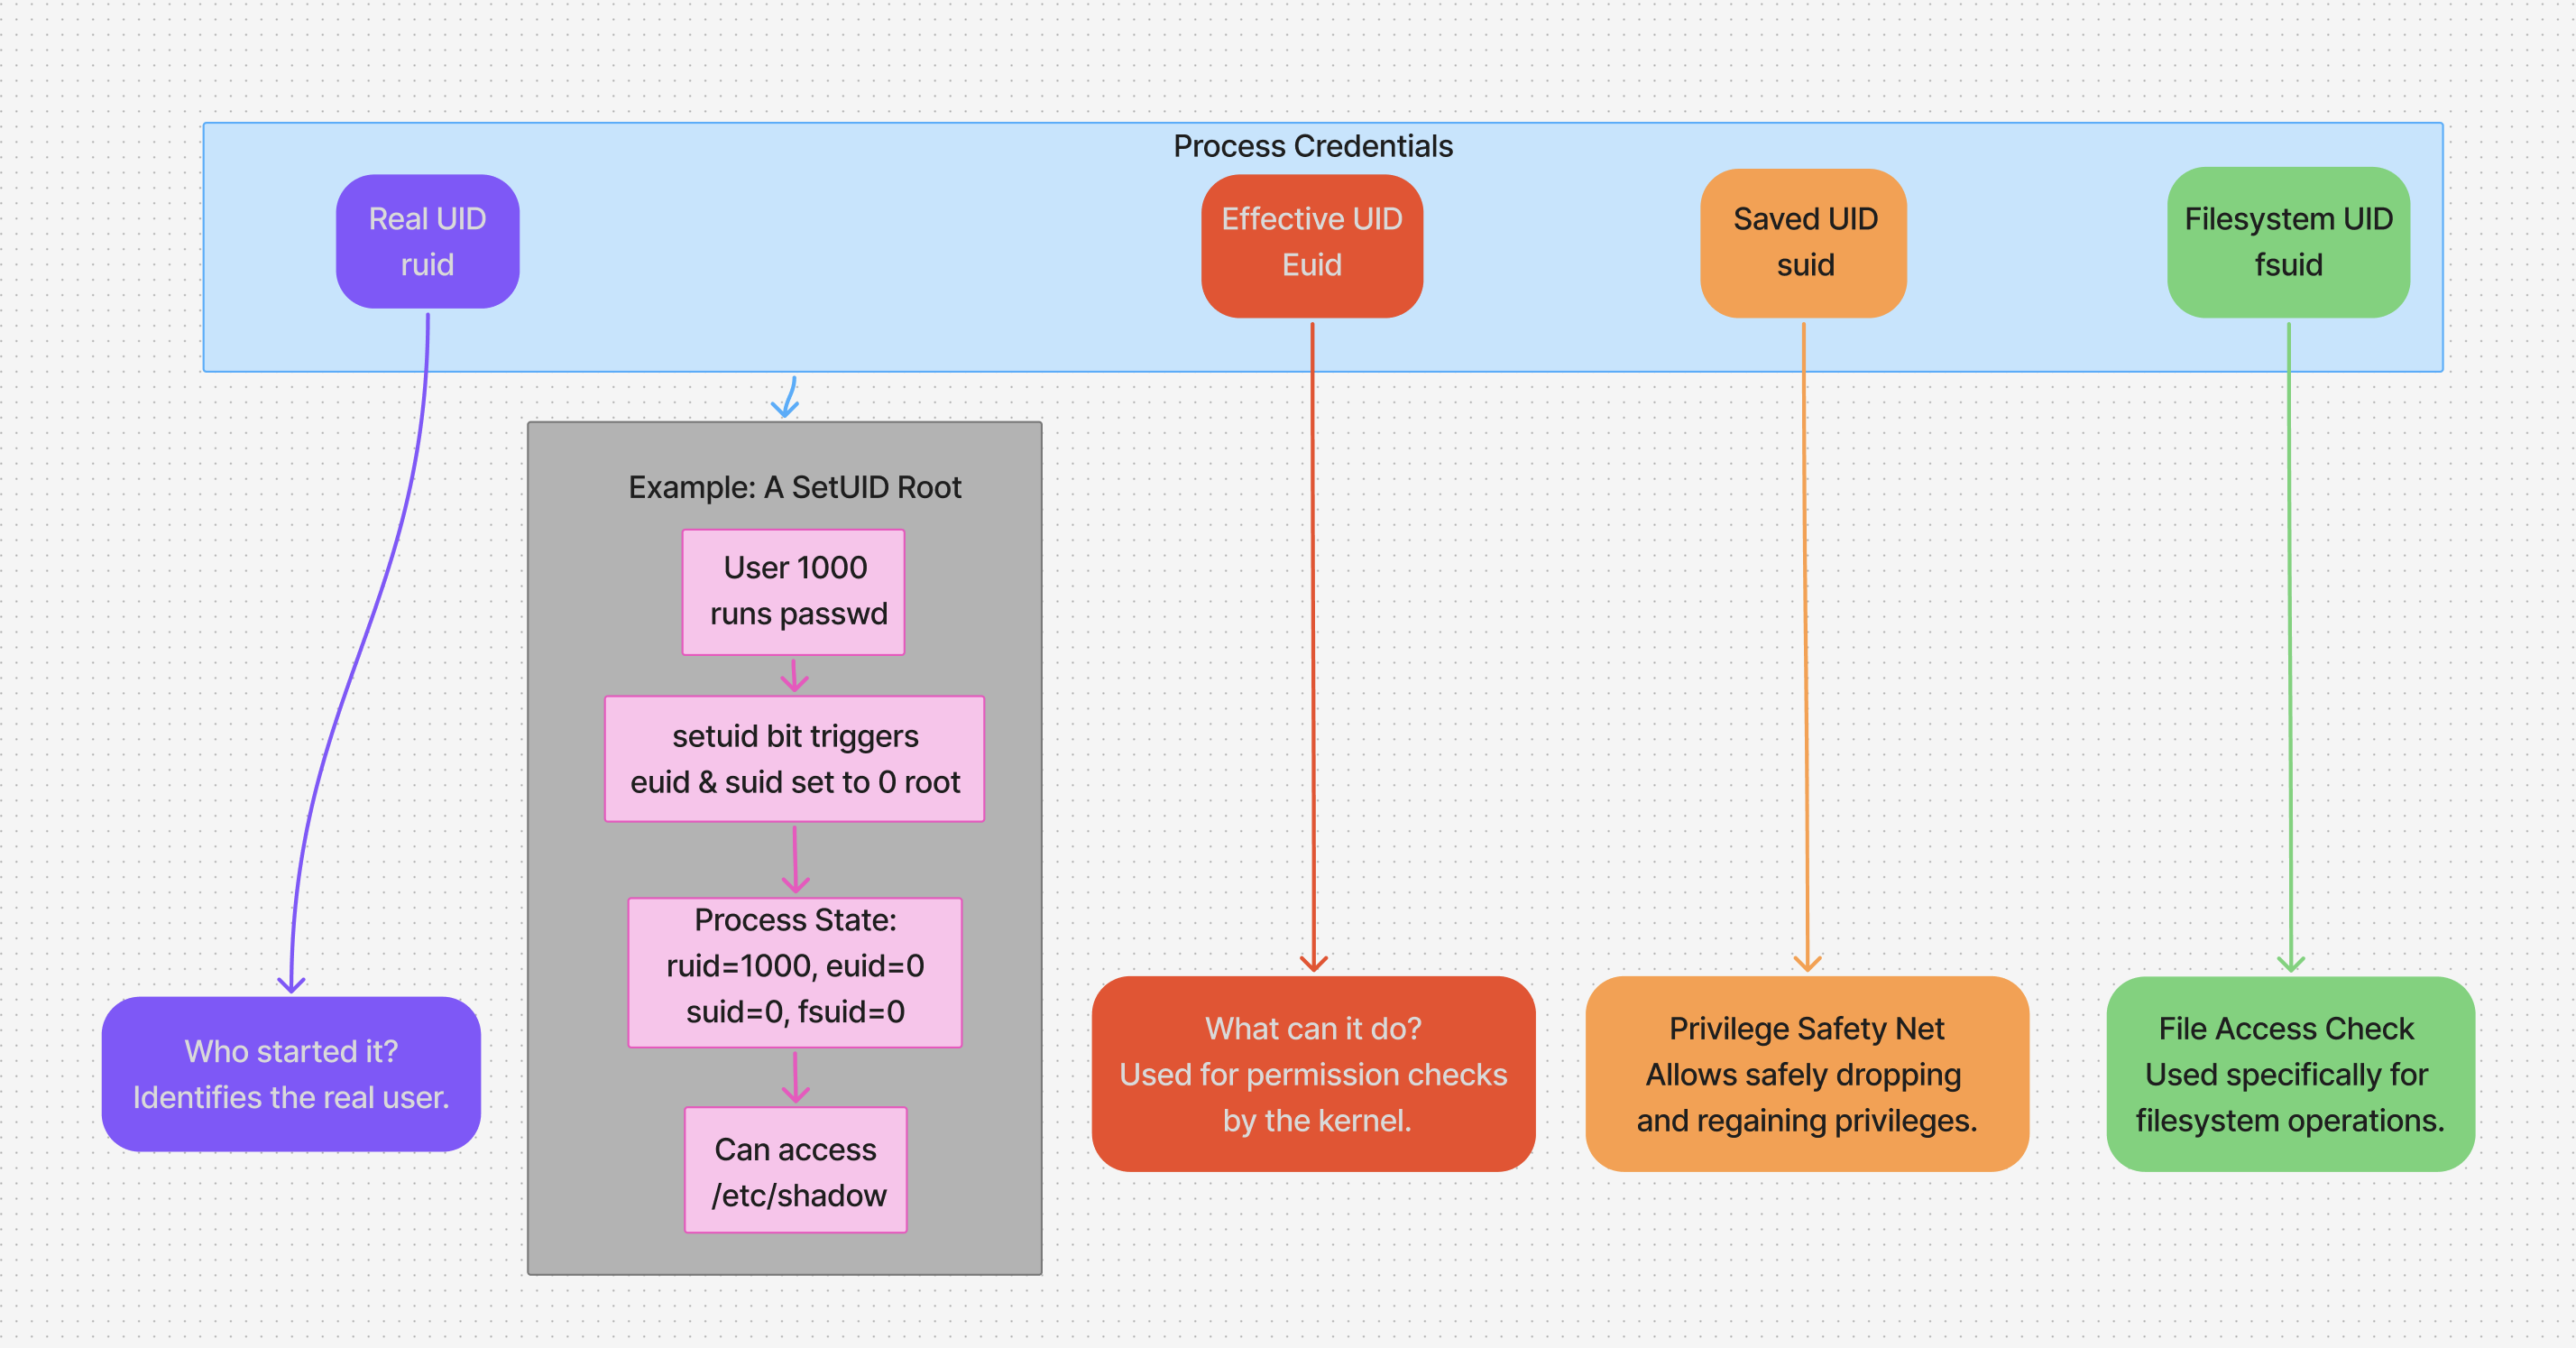
\includegraphics[
            width=0.85\textwidth,
            keepaspectratio
        ]{figures/chapter4/real_effective_saved_uid.png}
    }
    \caption[Real, Effective, Saved and Filesystem UIDs]
    {Real, effective, saved and filesystem UIDs for a process \cite{gazestani2025linuxuids}.}
    \label{fig:real-effective-saved-uid}
\end{figure}

Monitoring all these values is security-relevant because a process may change
its effective or filesystem privileges without changing its real identity.
Saved identities may also allow privileges to be regained after an apparent
drop. Observing only the real ID would therefore hide important transitions in
the process's effective authority \cite{gazestani2025linuxuids}.

Explicit identity requests are captured through the \texttt{setuid},
\texttt{setgid}, \texttt{setreuid}, \texttt{setregid},
\texttt{setresuid}, \texttt{setresgid}, \texttt{setfsuid} and
\texttt{setfsgid} events. Their entry programs retain one, two or three
identifiers according to the syscall interface. This preserves the distinction
between single-ID changes, separate real and effective identities, complete
real/effective/saved transitions and filesystem-specific identities. The exit
programs append the value returned to the caller.

The return value cannot be interpreted uniformly across the family. Most
set-ID operations use a conventional status value, while \texttt{setfsuid} and
\texttt{setfsgid} return the previous filesystem identity. Preserving the
originating logical event is therefore necessary for user space to interpret
the result correctly.

The \texttt{security\_task\_fix\_setuid} hook adds the mediation-stage view. It
records the old and proposed real, effective, saved and filesystem UIDs,
together with a flag that distinguishes the set-ID operation category. The
eBPF program compares the two credential proposals and suppresses the event
when none of the monitored UID fields changes. Since the hook is observed
before installation and its result is not captured, the event describes the
transition examined by the security subsystem rather than a confirmed change.

No public \texttt{security\_task\_fix\_setgid} event is currently exposed.
Group-ID requests remain visible through the set-group syscall events, while
changes that become active are included in the broader
\texttt{commit\_creds} event.

The \texttt{commit\_creds} hook observes the point at which replacement
credentials become active for the current task. It reads both the currently
installed credentials and the replacement supplied by the kernel, converting
them into fixed-width snapshots. Each snapshot contains real, effective, saved
and filesystem user and group identifiers, the user-namespace identifier,
secure bits, and the inheritable, permitted, effective, bounding and ambient
capability sets.

Credential installation is a frequent kernel operation, and not every
invocation changes a field relevant to the monitor. The implementation
therefore compares the two snapshots before submission. Listing
\ref{lst:commit-creds-filter} shows this change-only emission strategy.

\begin{lstlisting}[
    language=C,
    basicstyle=\ttfamily\footnotesize,
    caption={Kernel-side suppression of unchanged credential snapshots
    (abridged).},
    label={lst:commit-creds-filter}
]
slim_cred_t old_slim = {};
slim_cred_t new_slim = {};

/* Identifiers, namespace, secure bits and capability
 * sets are copied into the two snapshots. */

if (old_slim.uid == new_slim.uid &&
    old_slim.gid == new_slim.gid &&
    old_slim.euid == new_slim.euid &&
    old_slim.egid == new_slim.egid &&
    /* Remaining monitored fields are compared here. */
    old_slim.cap_ambient == new_slim.cap_ambient)
    return 0;

save_to_submit_buf(&p.event->args_buf,
                   &old_slim, sizeof(slim_cred_t), 0);
save_to_submit_buf(&p.event->args_buf,
                   &new_slim, sizeof(slim_cred_t), 1);

return events_perf_submit(&p);
\end{lstlisting}

The comparison occurs before the event enters the perf-event channel. Unchanged
credential installations therefore consume neither transport bandwidth nor
user-space decoding work. When a relevant difference is found, both snapshots
are preserved, allowing the transition to be analysed without reconstructing
the previous state from an earlier event.

The final observation point is \texttt{cap\_capable}. This event records the
capability number presented during a kernel capability check, exposing the use
of privilege-sensitive operations even when no credential replacement occurs.
A capability check is not equivalent to a privilege change or a successful
operation: the current schema does not retain the checked credentials, user
namespace, option flags or final decision.

Together, these events distinguish four forms of evidence: an explicit
identity request, a proposed transition under security mediation, the
credential state installed by the kernel and a later capability check. This
prevents the monitoring pipeline from treating all privilege-related activity
as the same kind of event.

\subsubsection{Process Control and Limits}
\label{subsubsec:implementation-process-control-limits}

Process-control operations can alter another task, modify the behaviour of the
current process or change the limits within which it executes. These operations
are security-relevant because they may support inspection, interference,
persistence or resource manipulation. The implementation observes them at
different boundaries according to where their most useful evidence becomes
available.

Cross-process control is represented by \texttt{ptrace} and
\texttt{security\_task\_kill}. The \texttt{ptrace} entry program retains the
request code, target PID and the address and data arguments supplied by the
caller. These pointer values are deliberately treated as opaque: the eBPF
program does not copy the memory to which they refer. At syscall exit, the
stored request is combined with the return value, allowing user space to
distinguish an accepted request from an error.

Signal delivery is observed through \texttt{security\_task\_kill}. The common
event context already identifies the source task, while the event-specific
payload describes the destination through its host PID and TID, UID and command
name. The signal number completes the source--operation--target relation.
Signal zero is retained because it can be used to test whether a target exists
and whether the caller has permission to signal it, even though no signal is
actually delivered.

Listing~\ref{lst:security-task-kill-relation} shows how the destination identity
is extracted from the target task rather than inferred from a caller-supplied
numeric PID.

\begin{lstlisting}[
    language=C,
    basicstyle=\ttfamily\footnotesize,
    caption={Target evidence collected by
    \texttt{security\_task\_kill} (abridged).},
    label={lst:security-task-kill-relation}
]
u32 target_pid = get_task_host_tgid(target);
u32 target_tid = get_task_host_pid(target);
u32 target_uid = 0;
char target_comm[TASK_COMM_LEN] = {};

const struct cred *target_cred =
    get_task_real_cred(target);
if (target_cred)
    target_uid = BPF_CORE_READ(target_cred, uid.val);

if (bpf_probe_read_kernel_str(
        target_comm, sizeof(target_comm),
        target->comm) <= 0)
    return 0;

save_to_submit_buf(&p.event->args_buf,
                   &target_pid, sizeof(u32), 0);
save_to_submit_buf(&p.event->args_buf,
                   &target_tid, sizeof(u32), 1);
save_to_submit_buf(&p.event->args_buf,
                   &target_uid, sizeof(u32), 2);
save_str_to_buf(&p.event->args_buf, target_comm, 3);
save_to_submit_buf(&p.event->args_buf,
                   &sig, sizeof(int), 4);
\end{lstlisting}

Reading the destination directly from its kernel task structure avoids relying
only on an identifier supplied by user space. However, this hook runs during
security mediation and does not expose the final decision or confirm that the
signal was delivered. It records an attempted relation rather than a completed
state change.

Changes to the current task's behaviour are monitored through
\texttt{security\_task\_prctl} and \texttt{do\_sigaction}. The former records
the requested \texttt{prctl} option and its four machine-word arguments. The
eBPF program intentionally leaves option-specific interpretation to user space,
avoiding a large command-dependent parser in kernel space.

The \texttt{do\_sigaction} event focuses specifically on signal-handler state.
It records the signal number, whether a new action was supplied and whether the
caller requested the previous action. For both the proposed and currently
installed actions, it captures the flags, first signal-mask word and handler
category or address. This makes changes such as installing, replacing or
ignoring a handler observable. Since the hook is attached at function entry,
the event does not confirm that the proposed action was installed.

Resource-limit monitoring combines a mediation view with syscall-level
outcomes. The \texttt{security\_task\_setrlimit} hook receives the resolved
target task and proposed kernel \texttt{rlimit} structure. It records the target
host PID, resource identifier, soft limit and hard limit while the operation is
being checked. It does not include the final decision.

The paired \texttt{prlimit64} event instead preserves the target PID, resource
identifier, addresses of the new and old user-space limit structures, and the
syscall return value. The pointed-to structures are not dereferenced by this
event. These two observations are therefore complementary: the security hook
exposes the proposed kernel values, while the syscall event preserves the
request interface and its reported outcome.

Finally, \texttt{security\_settime64} observes attempts to modify the system
clock. It records the proposed seconds and nanoseconds together with the
timezone offset and daylight-saving field. Changing wall-clock time is
privilege-sensitive and can affect timestamp-based analysis, for example an attacker 
can leverage the time modification to obscure their activities or perform some time 
based TOTP authentication, but this mediation-stage event does 
not by itself establish that the new time was installed.

This design keeps cross-process relations, task configuration and resource
changes as separate forms of evidence. Syscall return events provide explicit
outcomes where available, while security hooks expose resolved kernel objects
and proposed values without being treated as confirmation of success.

\subsection{File and Filesystem Security}
\label{subsec:implementation-filesystem-hooks}

Filesystem monitoring must distinguish the name supplied by a process from the
object eventually reached by the kernel. A pathname may be relative, interpreted
from a directory file descriptor or contain symbolic links. The Virtual File
System resolves these elements before operating on the corresponding filesystem
object \cite{linuxPathnameLookup}.

The implementation therefore combines two complementary perspectives.
Syscall probes preserve the original request and its returned result, while
security hooks observe objects that have already undergone kernel pathname
resolution. Where available, the resolved device and inode numbers provide a
local object identity, since an inode number is unique only within its
filesystem \cite{linuxInodeIdentifiers}.

The \texttt{open} event provides the syscall-level perspective. Entry probes for
\texttt{open} and \texttt{openat} retain the operation variant, directory file
descriptor, requested pathname, flags and creation mode. Exit probes add either
the returned file descriptor or a negative error. The two syscall variants
therefore share one logical schema without losing the differences between their
calling conventions.

The same design is used for filesystem metadata changes. The \texttt{chmod}
event monitors requests to modify permission bits, which determine whether an
object may be read, written or executed. It combines \texttt{chmod},
\texttt{fchmod} and \texttt{fchmodat}, recording the relevant pathname,
descriptor or directory-relative context, the requested mode and the syscall
result.

The \texttt{chown} event monitors requests to replace the user or group ownership
of an object. It combines \texttt{chown}, \texttt{fchown},
\texttt{fchownat} and \texttt{lchown}, retaining the requested owner and group
identifiers, pathname or descriptor context, flags and returned result.
The operation identifier remains important because \texttt{lchown} changes the
ownership of a symbolic link itself rather than following the link to its
target.

This consolidation separates the public event model from physical attachment.
Six entry and exit programs produce the single \texttt{chmod} event, while
eight produce \texttt{chown}. A compact operation field identifies the
originating syscall and avoids duplicating otherwise similar event schemas.

The syscall view is complemented by \texttt{security\_file\_open}. This hook is
invoked while the kernel is opening a file, after the Virtual File System has
resolved the pathname and constructed a \texttt{struct file}. Linux Security
Modules may use this stage to preserve open-time security state and re-evaluate
conditions previously checked through \texttt{inode\_permission}
\cite{linuxKernelSecurityFileOpen}. The hook therefore exposes the resolved
object under security inspection, but does not report the final LSM decision or
syscall result.

From the supplied \texttt{struct file}, the program obtains the resolved
pathname, file flags, device number, inode number and change time. When the
originating syscall is recognised, it also attempts to recover the pathname
argument from the current task register state. Listing
\ref{lst:security-file-open-paths} shows the essential separation between these
two forms of evidence.

\newpage

\begin{lstlisting}[
    language=C,
    basicstyle=\ttfamily\footnotesize,
    caption={Requested and resolved evidence collected by
    \texttt{security\_file\_open}.},
    label={lst:security-file-open-paths}
]
void *resolved = get_path_str(&file->f_path);
dev_t device = get_dev_from_file(file);
unsigned long inode = get_inode_nr_from_file(file);

void *requested = "";
struct pt_regs *regs = get_current_task_pt_regs();

if (p.event->context.syscall == SYSCALL_OPEN)
    requested = get_syscall_arg1(p.event->task, regs, false);
else if (p.event->context.syscall == SYSCALL_OPENAT)
    requested = get_syscall_arg2(p.event->task, regs, false);

save_str_to_buf(&p.event->args_buf, resolved, 0);
save_to_submit_buf(&p.event->args_buf, &device, sizeof(device), 2);
save_to_submit_buf(&p.event->args_buf, &inode, sizeof(inode), 3);
save_str_to_buf(&p.event->args_buf, requested, 5);
\end{lstlisting}

The requested and resolved paths answer different questions. The first
describes how the process referred to the file; the second describes the path
reconstructed from the kernel object. They may differ because of symbolic
links, relative traversal or mount topology. Requested-path recovery is
best-effort and may produce an empty value when the syscall or register state
cannot be identified. The resolved object remains available directly through
the \texttt{struct file}.

Path reconstruction is itself constrained by the eBPF execution model. The
implementation walks kernel dentries backwards and assembles the path in
per-CPU scratch storage rather than on the restricted eBPF stack. The traversal
is bounded to 20 components and a 4096-byte working region, allowing the
verifier to establish finite execution and memory bounds. Deep or disconnected
paths may consequently produce a partial or explicitly disconnected
representation. A resolved pathname must therefore be understood as bounded
kernel evidence rather than an unconditional canonical path.

Device and inode values provide a more stable local correlation key than a
pathname alone. Detectors can associate observations generated by different
processes when they refer to the same \texttt{device:inode} pair, even if the
path strings differ. The pathname remains useful as a detector condition, but
does not define resource identity. This correlation is deliberately local and
time-bounded because inode values can eventually be reused and layered
filesystems may expose different identities for apparently equivalent paths.

Further file hooks observe access checks and control requests on resolved
objects. \texttt{security\_file\_permission} records the pathname,
device-inode identity, change time and permission mask presented during a
read, write or execution check. It shows that the check occurred, but does not
establish whether access was ultimately granted. This is also a high-volume
observation point, making selective event activation particularly important.

The \texttt{security\_file\_ioctl} event monitors file and device-specific
control requests. It records the resolved target identity, ioctl command and
argument value. The argument is intentionally retained as an opaque value:
its interpretation depends on both the command and the target device, and
decoding every possible structure inside eBPF would increase complexity and
verifier cost.

Directory-entry hooks preserve objects at the point where their namespace
representation may change. \texttt{security\_inode\_unlink} records the path,
device, inode and change time of an entry proposed for removal. Capturing this
identity before the unlink operation is valuable because the pathname may no
longer resolve afterwards.

The \texttt{security\_inode\_rename} event records the old and new paths,
rename flags and the identity of the source object. Its implementation also
reveals a consequence of bounded per-CPU storage. Both paths are reconstructed
through the same scratch buffer, so the source path must be serialised into the
event before reconstruction of the destination begins. Otherwise, the second
traversal would overwrite the first result.

Creation-related hooks retain evidence specific to the new directory entry.
\texttt{security\_inode\_symlink} records the pathname of the symbolic link and
the caller-supplied target string, which may be relative or may not yet identify
an existing object. \texttt{security\_inode\_mknod} records the pathname,
requested mode and device number of a new special node. The mode identifies the
object type and permission bits, while the device number is meaningful for
character and block devices. Both events observe security mediation and do not
contain a final syscall result.

Mount hooks extend monitoring from individual objects to filesystem topology.
\texttt{security\_sb\_mount} records the source name, resolved target path,
filesystem type and mount flags. The filesystem-specific data argument is not
copied because its format varies between filesystems and may contain sensitive
configuration. \texttt{security\_sb\_umount} records the resolved mountpoint,
filesystem type and unmount flags. As entry observations of security hooks,
these events show that the requested topology change reached mediation, not
that it completed successfully.

The resulting implementation preserves three distinct forms of filesystem
evidence: the operation requested by a process, the kernel object involved in
security mediation and, for paired syscall probes, the result returned to the
caller. Keeping these stages separate prevents a pathname request or an LSM
observation from being presented as proof that the corresponding filesystem
operation succeeded.

\subsection{Memory, Namespace and Cgroup Transitions}
\label{subsec:implementation-memory-namespace-hooks}

Memory, namespaces and cgroups control different aspects of process execution.
Memory mappings determine which regions a process may access and how they may
be used. Namespaces determine which kernel resources a process can observe,
while cgroups define its position within a resource-control and accounting
hierarchy. Monitoring these mechanisms is security-relevant because they are
involved in code loading, process-memory access and changes to isolation
boundaries.

\begin{figure}[H]
    \centering
    \makebox[\textwidth][c]{%
        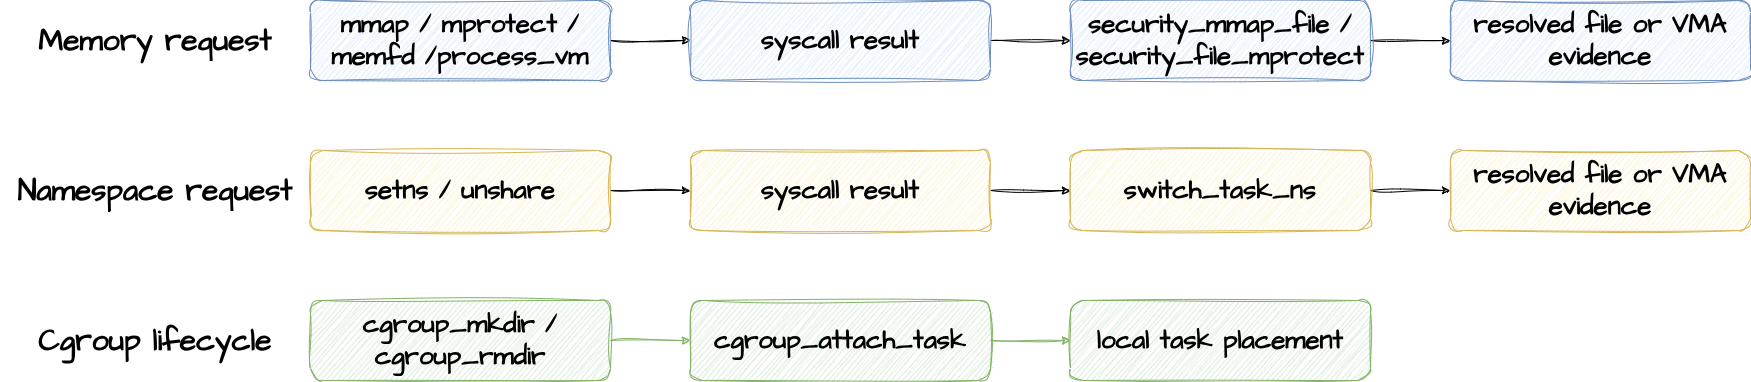
\includegraphics[
            width=1.20\textwidth,
            keepaspectratio
        ]{figures/chapter4/memory_namespace_cgroup_monitoring.drawio.png}
    }
    \caption[Memory and isolation transition monitoring]
    {Observation points used for memory operations, namespace transitions and
    local cgroup changes.}
    \label{fig:memory-namespace-cgroup-monitoring}
\end{figure}

Figure~\ref{fig:memory-namespace-cgroup-monitoring} represents complementary
observation paths rather than a mandatory sequence. A memory syscall may not
reach the corresponding security hook, and a successful namespace-related
syscall does not necessarily modify every namespace represented by the
committed-state event.

The \texttt{memfd\_create} event monitors the creation of an anonymous,
RAM-backed file. Such an object initially has no conventional filesystem
pathname, but it may later be mapped into memory or used as an executable
image. The event records the requested name and creation flags, followed by
the returned file descriptor or a negative error. This makes successful
anonymous-file creation distinguishable from a failed attempt without
requiring the monitor to inspect its future contents.

The \texttt{mmap} event records requests to create or modify mappings in a
process address space. Its entry probe retains the requested address, length,
protection mask, mapping flags, file descriptor and offset. The exit probe
adds either the address selected by the kernel or a negative error. These
fields distinguish anonymous mappings from file-backed mappings and identify
requests that combine writable and executable permissions.

The \texttt{mprotect} event monitors requests to change the permissions of an
existing memory range. It records the starting address, length, requested
protection mask and returned status. The related
\texttt{pkey\_mprotect} event additionally records the protection key assigned
to the range. Protection-key support is dependent on the target architecture
and kernel configuration, so the returned value remains necessary for
distinguishing an applied request from an unsupported or rejected operation.

The syscall events describe the process request, but they do not identify the
resolved kernel objects examined during security mediation. \\ The
\texttt{security\_mmap\_file} hook complements \texttt{mmap} for file-backed
mappings. It records the resolved pathname, file flags, device, inode, change
time, requested protections and mapping flags. Anonymous mappings are omitted
because no backing \texttt{struct file} is available; they remain visible
through the syscall event.

The \texttt{security\_file\_mprotect} hook observes a protection change through
the virtual memory area supplied by the kernel. It preserves three distinct
protection values: the permissions requested by user space, the permissions
adjusted by the kernel for security evaluation, and the access bits currently
installed on the region. It also records the region start and length. When the
mapping is file-backed, the event adds its resolved pathname and
device-inode identity; anonymous regions retain the protection and address
evidence without file metadata.

This distinction makes the event more informative than the syscall request
alone. It can show, for example, that a previously writable region is being
evaluated for executable access and whether that region is associated with a
resolved file. Since the probe observes entry to the security hook, however,
it does not contain the hook decision or the final syscall result.

The implementation reads the supplied virtual memory area directly. It does
not perform an independent search through the process memory-management tree.
This keeps the collection path bounded and avoids duplicating work already
performed by the kernel before invoking the security hook.

Cross-process memory access is monitored through
\texttt{process\_vm\_readv} and \texttt{process\_vm\_writev}. These events
record the target PID, addresses and element counts of the local and remote
I/O-vector arrays, operation flags and the number of bytes transferred or the
returned error. The vector elements and transferred memory contents are not
copied. This retains evidence that one process accessed another process's
address space while limiting overhead and avoiding collection of potentially
sensitive payload data.

Namespace events monitor changes to the resource views associated with a
process. The \texttt{setns} syscall requests that the caller join an existing
namespace referenced by a file descriptor. Its event records the descriptor,
the requested namespace type and the returned result. A type value of zero
allows the kernel to infer the namespace type from the descriptor.

The \texttt{unshare} syscall instead requests that selected execution-context
resources cease to be shared with other processes. Its event records the
complete \texttt{CLONE\_*} flag mask and the syscall result. Together,
\texttt{setns} and \texttt{unshare} distinguish entry into an existing
namespace from the creation or separation of an execution context.

A successful syscall result confirms that the request was accepted, but does
not directly expose the identifiers installed in the task. The
\texttt{switch\_task\_ns} event supplies this state-level perspective by
observing \texttt{switch\_task\_namespaces}, where the kernel replaces the
task's namespace proxy.

The hook compares the old and proposed namespace sets and emits an event only
when at least one monitored identifier changes. The record contains the task
PID and only the new identifiers for the changed mount, PID-for-children, UTS,
IPC, network or cgroup namespaces. Unchanged fields are omitted from the
indexed argument stream, keeping the record sparse and suppressing no-op
transitions. User namespaces are not part of this namespace-proxy comparison;
credential-related user-namespace changes are observed separately through the
credential hooks.

Cgroup monitoring addresses task placement rather than namespace replacement.
A cgroup namespace changes how a hierarchy is presented to a process, whereas
cgroup attachment changes the hierarchy node to which the task belongs. The
implementation preserves this distinction.

The \texttt{cgroup\_attach\_task} raw tracepoint reports movement of a task to
a destination cgroup. It records the destination cgroup and hierarchy
identifiers, the supplied cgroup path, target command name, host PID and TID,
and whether the operation concerns the complete thread group. This allows the
monitor to observe containment changes even when the task identity itself
remains unchanged.

The \texttt{cgroup\_mkdir} and \texttt{cgroup\_rmdir} events describe the
lifecycle of the local cgroup hierarchy. Both retain the cgroup identifier,
bounded path and hierarchy identifier supplied at creation or removal. They do
not reconstruct a persistent hierarchy in user space; each event represents a
local lifecycle observation.

Cgroup identifier extraction also contains a compatibility decision specific
to the supported kernel range. The layout of the underlying
\texttt{kernfs\_node} identifier differs between older kernels, newer kernels
and the hidden KABI representation used by the target RHEL-derived kernel.
CO-RE field-existence checks select the available layout at load time, allowing
the same helper to obtain the identifier without hard-coding a single
structure version.

Namespace inode numbers and cgroup identifiers remain local kernel identities.
They are useful for comparing events and for detector correlation on one node,
but they are not interpreted as pod, container or cluster-wide workload
identifiers. The implementation therefore provides evidence of local memory
and isolation transitions without claiming to reconstruct a persistent
namespace graph, cgroup hierarchy or Kubernetes execution model.

\subsection{Kernel Integrity and Kernel-Facing Activity}
\label{subsec:implementation-kernel-activity-hooks}

Kernel modules, eBPF objects and dynamic instrumentation can modify or inspect
behaviour inside the kernel. These mechanisms are legitimate parts of Linux,
but they also expose high-impact interfaces whose use is relevant to runtime
security monitoring. The implemented hooks preserve the operation, object
identity and result available at each observation point. They provide evidence
for subsequent detectors and do not classify an operation as malicious by
themselves.

Kernel-module monitoring separates lifecycle notifications from module
initialisation results. The \texttt{module\_load} raw tracepoint records a
module as it enters the kernel module lifecycle, while
\texttt{module\_free} reports its removal. Both events preserve the module
name and, when available, its version and source-version strings. They do not
copy module code, sections or other internal contents.

These lifecycle events do not indicate whether the module's initialisation
function completed successfully. The \texttt{do\_init\_module} event therefore
uses a kprobe and kretprobe pair. At function entry, the module object is
retained in per-thread temporary state. At return, the implementation retrieves
that object, extracts the module identity and appends the function result. A
zero value identifies successful initialisation, while a negative value
preserves the reported kernel error.

This distinction prevents a module observed during loading from being
automatically treated as operational. The lifecycle tracepoints identify
additions and removals, whereas \texttt{do\_init\_module} provides the outcome
of the initialisation stage. These events can later be correlated without
assigning a security meaning to ordinary module-management activity.

The eBPF hooks observe a different kernel-facing interface. They are kprobes
attached to Linux Security Module functions invoked while eBPF commands and
objects undergo security checks. They are not themselves BPF LSM enforcement
programs and do not modify the kernel's decision.

The \texttt{security\_bpf} hook monitors operations entering the security path
of the \texttt{bpf} syscall. Its purpose is to expose requests such as map
creation, program loading and program attachment. The event records the BPF
command and attribute size, but does not copy \texttt{union bpf\_attr}, whose
active fields depend on the command.

The \texttt{security\_bpf\_map} hook observes security checks involving an
existing eBPF map. Since maps retain state and exchange data between kernel
programs and user space, identifying access to them provides useful
object-level evidence. The event records the map identifier and bounded name,
without collecting its contents.

The \texttt{security\_bpf\_prog} hook observes security operations involving an
existing eBPF program. It records the program identifier, name and type,
allowing programs intended for kprobes, tracepoints, cgroups and other
execution contexts to be distinguished.

Together, these hooks identify the requested BPF operation and the map or
program involved in security mediation.

\subsubsection{Dynamic Instrumentation and Kernel Interfaces}
\label{subsubsec:implementation-dynamic-instrumentation}
Dynamic instrumentation and kernel-facing interfaces expose activity that is
not always visible through ordinary process syscalls. The following events
monitor selected interfaces used for tracing, symbol resolution, procfs
creation, kernel-initiated execution and kernel file consumption.

The \texttt{register\_kprobe} event monitors attempts to install dynamic
kprobes. It records the target symbol, pre- and post-handler addresses, and
registration result. This distinguishes successful installations from rejected
requests, although the symbol may be absent when registration uses a kernel
address directly.

The \texttt{kallsyms\_lookup\_}\allowbreak\texttt{name} event monitors kernel
symbol resolution. It combines the requested symbol name with the returned
address, where zero indicates that no address was found. It covers this
specific lookup interface rather than every possible source of kernel
addresses.

The \texttt{proc\_create} event observes requests to create procfs interfaces.
It records the entry name and proc-operations address, making kernel-created
user-space control or information endpoints visible. It does not include the
parent directory, complete path or creation result.

The \texttt{call\_usermodehelper} event monitors requests by the kernel to start
a user-space program. It records the executable path, bounded argument and
environment arrays, and wait mode. The arrays contain at most 38 elements and
remain subject to the event-size limit. The event represents the request, not
successful execution or completion of the helper.

The \texttt{security\_kernel\_read\_file} event observes the security stage
before the kernel consumes a file. It records the resolved pathname, device,
inode, change time and read purpose, distinguishing uses such as modules,
firmware, policy data and kexec images.

The later \texttt{security\_kernel\_post\_read\_file} event records the same
file identity and purpose together with the supplied byte size. This size is
not a return value. The two stages are emitted independently: the
implementation does not correlate them automatically, copy file contents or
compute a digest.

Together, these hooks expose selected instrumentation, procfs,
kernel-initiated execution and kernel-file activity. They do not inspect
handler code, reconstruct every kernel relationship, prove integrity or
enforce a security decision. The following section explains how these logical
events activate their physical probes and support dependencies.

\section{Loader, Probe Registry and Attachment Lifecycle}
\label{sec:implementation-loader-registry}

Runtime construction begins after configuration and external rule documents
have been accepted. Object resolution gives precedence to an environment
override, then to an explicit path, and finally to the embedded object produced
in Section~\ref{sec:implementation-build-organisation}. BTF resolution is
independent and similarly permits an environment or configuration override
before using \path{/sys/kernel/btf/vmlinux}.

The effective logical-event set is established before the object is loaded.
The probe registry converts that set into program specifications containing the
compiled program name, physical hook, attachment kind and implied internal
dependencies. Public producers correspond to selectable decoder events,
whereas internal specifications supply state or enrichment without appearing
in event listing. Listing~\ref{lst:probe-dependency-expansion} shows the
selection loop that admits direct producers and dependencies implied by the
selected public events.

\begin{lstlisting}[
    caption={Go expansion from selected logical events to producer and support probes.},
    label={lst:probe-dependency-expansion}
]
selectedProbes := make([]Spec, 0, len(supportedProbes))
for _, probe := range supportedProbes {
    if _, ok := selectedEvents[probe.eventName]; ok {
        selectedProbes = append(selectedProbes, probe)
        continue
    }
    for _, trigger := range probe.impliedBy {
        if _, ok := selectedEvents[trigger]; ok {
            selectedProbes = append(selectedProbes, probe)
            break
        }
    }
}
\end{lstlisting}

This expansion makes attachment planning depend on the registry rather than
on naming conventions in the loader. One logical event may retain several
producer programs, while an internal program is added only when one of its
declared triggers is selected. The resulting program set is then used to
disable autoload for unrelated registered sections before object loading.

Before libbpf loads the object, autoload is disabled for registered programs
outside the resolved selection. Verification and relocation are consequently
avoided for those registered sections. This optimisation is bounded by the
registry: a program omitted from it cannot be disabled through this planning
step, so registry completeness is part of the loading correctness boundary.

After object loading, the runtime updates configuration maps, creates the perf
reader and attaches each selected program according to its registry kind. Raw
tracepoints, tracepoints, kprobes and kretprobes use their corresponding
libbpfgo attachment paths. Every successful attachment is retained as an owned
link.

The active loop consumes perf records until cancellation. Shutdown destroys
links in reverse acquisition order, releases any runtime-managed cgroup mount,
closes the perf reader and then closes the loaded module. This order preserves
resource ownership across partial initialisation and normal shutdown.

\section{Binary Event Contract and Kernel Transport}
\label{sec:implementation-binary-contract}

An ordinary event record consists of a 136-byte common context, a one-byte
argument count and a variable stream of indexed arguments. The Go context
mirrors the C field order explicitly. This fixed boundary is followed by only
the bytes actually used in the argument buffer, so a short event does not
transport the full 32,000-byte workspace.

Each argument starts with its one-byte schema index. A scalar payload follows
at the width defined by the event registry. Variable-length values add a
four-byte size field before their content, while string and compact argument
arrays use bounded sub-records. No independent wire type tag is transmitted.
The index selects the name and type from the user-space schema, allowing
arguments that could not be captured to be omitted without changing the
identity of later arguments.

The argument writer must expose an upper bound to the verifier without changing
a valid offset. Listing~\ref{lst:argument-buffer-bounds} presents the relevant
part of the write path.

\begin{lstlisting}[
    language=C,
    caption={Checked argument-buffer offset handling (abridged).},
    label={lst:argument-buffer-bounds}
]
if (size == 0 || size > MAX_ELEMENT_SIZE || buf->offset >= ARGS_BUF_SIZE)
    return 0;
u32 offset = buf->offset;
update_min(offset, ARGS_BUF_SIZE - 1);
u32 buffer_index_offset = offset + 1;
if (buffer_index_offset > ARGS_BUF_SIZE)
    return 0;
buf->args[offset] = index;
// The omitted block clamps size for the older verifier.
u32 buffer_arg_offset = buffer_index_offset + size;
if (buffer_arg_offset > ARGS_BUF_SIZE)
    return 0;
if (bpf_probe_read(&(buf->args[buffer_index_offset]), size, ptr) < 0)
    return 0;
buf->offset = buffer_arg_offset;
buf->argnum++;
return 1;
\end{lstlisting}

The 32,000-byte capacity is not a power of two, so masking an offset with the
capacity minus one would fold valid positions onto earlier bytes. The helper
instead checks the original value and communicates its upper bound through
\texttt{update\_min}. The final offset is committed only after the complete
write succeeds, preserving the indexed stream consumed by the Go decoder. The
correction of this non-power-of-two bounds error is recorded by commit
\texttt{163ad724a65ec8c701dc816fe87f174eeec51275}.

At submission, the common helper enriches the task context, optionally records
a user-space stack identifier, computes the fixed and variable portions of the
record and calls \texttt{bpf\_perf\_event\_output} for the current CPU. The
\texttt{events} map is a perf-event array, and the Go runtime creates one
libbpfgo perf reader over it. No BPF ring-buffer transport path is retained in
the current implementation.

Per-CPU losses are reported through the reader's loss channel, while records
that arrive but fail structural decoding follow a separate diagnostic path.
The capacity and ordering implications of perf-event transport are discussed
in Section~\ref{subsec:perf-buffer-failure-boundaries}.

\section{User-Space Decoder and Event Registry}
\label{sec:implementation-decoder-registry}

The decoder reads the fixed context in little-endian field order, obtains the
argument count and resolves the numeric event identifier. Each argument index
selects its declaration and payload decoder from the event registry. Decoded
values are reordered according to that schema and returned as the typed event
consumed directly by policies and detectors. The output adapter introduced in
Section~\ref{sec:implementation-output-logging} is a presentation model, not a
second security-event normalisation stage.

The indexed wire format allows a producer to omit unavailable evidence without
renumbering later fields. The decoder therefore accumulates records by their
encoded index and reconstructs the public argument order only after all
available payloads have been interpreted. Listing~\ref{lst:decoder-indexed-arguments}
shows this schema-directed core. The unknown-event diagnostic and final
schema-order reconstruction are omitted.

\begin{lstlisting}[
    caption={Schema-directed reconstruction of indexed arguments (abridged).},
    label={lst:decoder-indexed-arguments}
]
spec, ok := events.GetSpec(eventID)
if !ok {
    return decodeUnknownArguments(rawArgs, eventID, argnum)
}
decoded := make(map[int]Argument, argnum)
offset := 0
for seen := 0; seen < argnum && offset < len(rawArgs); seen++ {
    index := int(rawArgs[offset])
    offset++
    if index >= len(spec.Args) {
        return nil, fmt.Errorf("argument index %d out of range for event %s", index, spec.Name)
    }
    argSpec := spec.Args[index]
    value, consumed, err := decodeArgRecord(rawArgs[offset:], argSpec.DecodeAs)
    if err != nil {
        return nil, fmt.Errorf("decode arg %d (%s) [event %d %s]: %w",
            index, argSpec.Name, eventID, spec.Name, err)
    }
    offset += consumed
    decoded[index] = Argument{
        Name:  argSpec.Name,
        Type:  argSpec.DecodeAs,
        Value: value,
    }
}
\end{lstlisting}

The temporary map belongs to one decode call. A later duplicate index replaces
the earlier value, after which the function emits only present entries in
schema order. The wire carries no independent type tag, so the selected schema
is both the decoding instruction and the type contract; malformed payloads are
contained as errors at this boundary rather than forwarded as partially typed
events.

The decoder rejects a truncated fixed context, unknown event identifiers,
argument indexes outside the selected schema, truncated scalar or variable
payloads, oversized variable-length fields and invalid UTF-8 in textual
payloads. Since the wire format carries no type tag, it cannot independently
compare a transmitted type with the schema: structurally incompatible data
fail during decoding, while byte-compatible data are interpreted as the
registered type.

The boundary is intentionally tolerant of partial event enrichment. Missing
arguments are accepted, and a duplicate index replaces the previous value for
that index. The implementation also does not require every trailing byte to be
consumed. The resulting guarantee is therefore bounded, schema-directed
interpretation rather than a unique canonical encoding. Unknown or
structurally unsafe records are diagnosed and discarded without terminating
the reader loop.

Consistency tests across the event and probe registries ensure that ordinary
public probes have decoder definitions,
decoder events are publicly producible, internal probes remain hidden, and
multi-probe families retain their expected composition. Numeric C and Go event
constants are still synchronised by maintenance discipline rather than by an
automated cross-language constant comparison, making this interface a notable
compatibility obligation.

\section{Event Selection and Kernel-Side Filtering}
\label{sec:implementation-selection-filtering}

During probe planning, CLI selection, explicit exclusions and any finite
policy-derived allow-list determine which registered programs retain autoload
and attachment. This changes the producer set before collection begins.

The exact effective-UID guard runs during common eBPF initialisation. User space
updates two fields in the singleton configuration map: an enable
flag and one 32-bit UID. When enabled, the program compares that value with the
effective UID returned for the current task and exits before complete context
enrichment and submission on a mismatch. This is a single equality filter. It
does not implement ranges, exclusion sets, namespace-aware identities or a
general kernel policy language.

Listing~\ref{lst:ebpf-early-admission} is the complete decision helper. Its
placement inside the shared initialiser makes the same narrow guard available
to every producer that uses the framework from
Section~\ref{subsec:implementation-shared-event-construction}.

\begin{lstlisting}[
    language=C,
    caption={Exact effective-UID admission guard.},
    label={lst:ebpf-early-admission}
]
statfunc bool should_drop_by_kernel_uid_filter(config_entry_t *config)
{
    if (config == NULL)
        return false;
    if (config->kernel_uid_filter_enabled == 0)
        return false;
    u32 current_uid = (u32) bpf_get_current_uid_gid();
    return current_uid != config->kernel_uid_filter;
}
\end{lstlisting}

A null configuration pointer or a disabled flag admits the event. When active,
only a mismatch is dropped; no state is retained by the helper and no
authorisation result is produced. The guard reduces construction and transport
for excluded effective UIDs, while richer admission remains a user-space
operation.

After decoding, the effective event set, command-name filter and typed policy
predicates form the user-space admission path. Rejected events reach neither
raw presentation nor detector dispatch. The later \texttt{alerts-only} control
suppresses raw presentation without bypassing detector evaluation.

The configuration-map update currently depends on an explicit C layout. The
Go runtime patches the filter-enable field at byte offset 12 and the UID at
byte offset 16 after checking the map value size. The complete C configuration
structure is not mirrored in Go, and no loaded-object integration test reads
these fields back. The offsets must consequently evolve together with the C
structure in the same way as the event contract.

\section{Policy and Detector Engine}
\label{sec:implementation-policy-detector}

Policy and detector paths may identify a YAML file or a directory. Directory
loading is non-recursive and sorted by filename, giving deterministic catalogue
construction. YAML documents are converted into internal definitions before
they are consumed. Policy conversion applies omitted mode and intent defaults
and compiles compact argument filters into internal predicates. Unsupported
compact forms are skipped, and the YAML decoders do not universally reject
unknown fields. At event time, scope is tested before alternative rules;
exclusions and matching suppress policies take precedence. An exact finite
policy allow-list may also narrow the logical-event set before probe loading,
as described in Section~\ref{sec:implementation-selection-filtering}.

Detector parsing validates structural metadata, referenced event names,
severity, time-window bounds, ATT\&CK identifier syntax and correlation
compatibility. Runtime construction then normalises field and operator names,
splits membership operands, parses numeric operands and compiles ordered steps
and the correlation plan. Equality, inequality, containment, membership,
prefix, suffix, existence, non-existence and numeric comparisons consequently
run without reparsing the YAML representation. The registry rejects invalid or
duplicate identities, and the dispatcher builds an event-name index once.
Only detectors interested in the admitted logical event are invoked; a failure
remains associated with its detector and does not stop the other candidates.

The stateless path evaluates global conditions and the event-specific
condition group, then creates an alert from that single evidence event. A
definition becomes an ordered stateful sequence only when it is marked
stateful and contains more than one compiled step. Otherwise, multiple steps
act as alternative event-specific groups rather than as temporal stages.

For the stateful path, each correlation key owns the index of the next expected
step, the first-observation time and the ordered evidence retained so far.
Listing~\ref{lst:collective-state-advance} shows expiry handling and successful
advancement for an existing key. Global-condition evaluation, key construction
and first-step creation are omitted from the excerpt.

\begin{lstlisting}[
    caption={Go state transition for a collective detector sequence (abridged).},
    label={lst:collective-state-advance}
]
for _, key := range lookupKeys {
    state, ok := d.state[key]
    if !ok {
        continue
    }
    if now.Sub(state.firstSeen) > window {
        delete(d.state, key)
        continue
    }
    matches, err := stepMatches(event, d.steps[state.nextStep])
    if err != nil {
        return nil, err
    }
    if matches {
        state.events = append(state.events, event)
        state.nextStep++
        if state.nextStep >= len(d.steps) {
            delete(d.state, key)
            return []detectors.Alert{d.newAlertFromEvents(state.events)}, nil
        }
        d.state[key] = state
        return nil, nil
    }
}
\end{lstlisting}

Completion deletes the partial sequence before creating its alert. An
intermediate transition writes the advanced state back, while a new first-step
match starts or replaces the one sequence allowed for its key. The correlation
plan is compiled into typed key components: process identity combines host PID
and start time; process-tree lookup adds only the immediate parent candidate;
resource identity requires device and inode without a pathname fallback; and
cgroup identity requires a non-zero local identifier. Composite strategies are
ordered conjunctions, so any missing component prevents key construction. The
unsupported \texttt{user\_session} strategy is rejected rather than
approximated from UID.

An omitted stateful window defaults to two seconds and cannot exceed five
seconds. Its deadline begins with the first observation and is not extended by
later progress. Each detector retains at most 4,096 incomplete keys and one
sequence per key; starting that key again replaces its previous state, while
capacity pressure evicts the oldest first observation. The addressed state is
checked for expiry on each relevant event, and unrelated state is scanned
opportunistically at intervals no longer than one second. \texttt{Flush}
removes expired entries without timeout alerts, but the main runtime does not
schedule it periodically, so idle expired entries may remain until later
activity or an external flush.

After evaluation, the engine deduplicates alerts over five seconds. Its key
uses detector identity, title and severity together with the first evidence
event's name, PID, UID, command and ordered arguments. Later evidence from a
collective match is not part of that key, so different completions sharing the
same first observation may be collapsed. This suppresses alert delivery only;
it does not alter admitted events or detector sequence state.

Finally, detector definitions may carry framework, version, tactic, technique,
data-source and data-component fields. Validation accepts unmapped detectors
and checks only the syntax of non-empty tactic and technique identifiers; no
external ATT\&CK catalogue is consulted and mappings are not inferred. When a
detector matches, its complete configured threat metadata is copied into the
evidence-bearing alert passed to Section~\ref{sec:implementation-output-logging}.

\section{Output and Structured Logging}
\label{sec:implementation-output-logging}

Independent event and alert printers support line-oriented JSON and compact
table formats on standard output. Operational diagnostics instead use the Zap
logger on standard error and do not participate in security-data
serialisation.

Before JSON rendering, a decoded event is adapted to a presentation record that
groups process, host and kernel metadata, converts fixed-size C strings and
retains typed arguments. Table output
selects a smaller set of fields and resolves selected numeric values, including
signals, capabilities, operation flags, file descriptors and error numbers,
into readable labels while retaining their numeric meaning.

An alert record contains detector identity, title, severity, timestamp,
metadata, ATT\&CK classification and the retained event evidence. Point-alert
table output includes a source-event summary. Collective-alert output instead
prints the ordered evidence sequence and avoids repeating its first event in
separate source fields. The rendered sequence is bounded to 1,024 characters
and is truncated with an ellipsis when necessary. Structured JSON preserves
the complete evidence representation supplied to the output adapter.

Operational diagnostics are implemented with Zap \cite{uber_zap}. The logger
supports console and JSON encodings and debug, info, warning and error
thresholds. It uses ISO-8601 timestamps, disables caller and stack-trace fields,
and writes to standard error. Runtime startup, attachment, transport loss,
decoding failures, detector failures, output errors and cleanup conditions use
this path.

Libbpf diagnostics enter through a callback and receive a structured source
field. Libbpf warnings are mapped to warning records; other admitted messages
are mapped to debug records. Combined callback and Zap level filtering keeps
CO-RE relocation detail available for diagnosis without mixing it into normal
event or alert output. Configuration errors that occur before logger creation
are returned to the command entry point and printed as a concise outer error
boundary.

\section{Containerisation and Deployment Considerations}
\label{sec:implementation-containerisation}

The Dockerfile uses a builder and a runtime stage. The builder is based on Go
1.22 and Debian Bookworm and installs the C, LLVM, libelf and zlib development
dependencies required by the same aggregate build used on the host. It copies
the complete source tree because the Go module replaces libbpfgo with the local
third-party checkout. The final Debian slim stage installs only the libelf and
zlib runtime libraries and copies the generated executable.

The final image does not need a separate eBPF object because that object is
embedded in the executable. In the current Dockerfile, however, the policy and
detector YAML catalogues are not copied into the runtime stage. A container
that uses those external definitions must therefore receive them through a
mounted path or be built from a derivative image that includes them. This is a
packaging boundary rather than an event-processing limitation.

The container continues to operate against the host kernel. The supplied run
target grants privileged execution, joins the host PID and cgroup namespaces,
and exposes host BTF and bpffs paths; it is not a least-privilege deployment
profile. The target does not mount tracefs or debugfs explicitly, so hosts on
which libbpf requires those paths for selected tracepoints need an additional
mount or an adjusted launch command.

No Kubernetes deployment resources are part of the repository; node-level
deployment and cluster-wide alert aggregation remain external integration work.

\section{Compatibility and Verifier Challenges}
\label{sec:implementation-compatibility-verifier}

CO-RE reads are combined with explicit compatibility branches rather than
being treated as a complete portability solution. Task PID access selects
between the older PID-link representation and the newer thread-PID field.
Task start-time extraction chooses among boot-time, real-start-time and
start-time fields according to field and helper availability. Capability reads
similarly support the older pair of 32-bit words and the newer 64-bit
representation.

The cgroup identifier path contains a dedicated branch for the hidden layout
used by the RHEL 8 kernel family, in addition to older and newer upstream
representations. Inode change-time extraction selects among the pre-6.6,
6.6--6.10 and later layouts. The virtual-memory lookup helper traverses the
red-black VMA tree only when that representation exists and does not
approximate support for later maple-tree kernels. This bounded helper remains
available in the shared source but is not invoked by the host memory hooks
described in Section~\ref{subsec:implementation-memory-namespace-hooks}; its
presence must therefore not be interpreted as evidence collected by those
events.

Helper availability also changes the implementation path. Current syscall
registers are obtained through BTF-aware task helpers when available. The
fallback derives the register frame from the task stack and is explicitly tied
to x86-64 assumptions: 4 KiB pages, a 16 KiB kernel stack and no KASAN stack
expansion. Compatible 32-bit tasks are identified through their thread status,
and their syscall numbers are translated through a dedicated map before event
classification.

Several numeric limits arise from verifier behaviour rather than from the
security model. Path reconstruction, string-array traversal and VMA lookup use
fixed loop bounds; variable buffer writes repeat explicit range checks after
helper calls; and the submitted record length is clamped through
verifier-visible operations. The shared syscall-exit path restricts the return
argument index to less than 16 because the target Rocky Linux verifier did not
accept the broader generic bound. Dedicated typed tracepoints are used for
selected memory syscalls to keep the target path simpler than the generic
dispatcher.

These branches adapt one object across compatible layouts but cannot provide
unavailable symbols, hooks, helpers or attachment mechanisms. As established
in Section~\ref{subsec:ebpf-btf-core}, the implementation therefore claims
compatibility with the identified Rocky Linux target rather than unconditional
portability across Linux versions.
